\documentclass[%
reprint,
%superscriptaddress,
%groupedaddress,
%unsortedaddress,
%runinaddress,
%frontmatterverbose,
%preprint,
%showpacs,preprintnumbers,
%nofootinbib,
%nobibnotes,
%bibnotes,
 amsmath,amssymb,
 aps,
%pra,
%prb,
%rmp,
%prstab,
%prstper,
%floatfix,
]{revtex4-2}

\usepackage{graphicx}% Include figure files
\usepackage{dcolumn}% Align table columns on decimal point
\usepackage{bm}% bold math
%\usepackage{hyperref}% add hypertext capabilities
%\usepackage[mathlines]{lineno}% Enable numbering of text and display math
%\linenumbers\relax % Commence numbering lines

%\usepackage[showframe, %Uncomment any one of the following lines to test
%scale=0.7, marginratio={1:1, 2:3}, ignoreall,% default settings
%text={7in,10in},centering,
%margin=1.5in,
%total={6.5in,8.75in}, top=1.2in, left=0.9in, includefoot,
%height=10in,a5paper,hmargin={3cm,0.8in},
%]{geometry}

%\usepackage[utf8]{inputenc}
%\usepackage[left=2.5 cm, right = 2.5 cm, top = 2.5 cm, bottom = %2cm, headheight=36pt]{geometry}
\usepackage{amsmath}
\usepackage{amssymb}
\usepackage{amsthm}
\usepackage{enumitem}
\usepackage{scrextend}
\usepackage{setspace}
\usepackage{fancyhdr}
\pagestyle{fancy}
\usepackage{siunitx}
%\usepackage[square,numbers]{natbib} 
%\bibliographystyle{abbrvnat}
%\usepackage{hyperref}
%\usepackage{cleveref}
%\usepackage{gensymb}


\begin{document}

\title{Worm algorithm for the Ising model}% Force line breaks with \\
%\thanks{A footnote to the article title}%

\author{Ajay S. Sakthivasan}
 \email{s6ajsakt@uni-bonn.de}
\author{Dongjin Suh}
 \email{s6dosuhh@uni-bonn.de}

\date{\today}% It is always \today, today,
             %  but any date may be explicitly specified

\begin{abstract}
In this project, we study the worm algorithm, a non-local algorithm proposed as an alternative to local algorithms like the Metropolis algorithm. Both the metropolis and the worm algorithm are implemented for the 2D Ising model, and results for large lattice sizes are extracted. The results include the behaviour of net magnetisation, magnetic susceptibility and heat capacity, autocorrelation times and the dynamical critical exponent. These are then compared. Particularly, the value of the dynamical critical exponent is discussed. Further, the drawbacks of the current implementations are discussed along with suggestions for direction of future work.
\end{abstract}
\maketitle

\tableofcontents

\section{Introduction} 
Monte Carlo methods are powerful numerical techniques for simulating complex systems. In the context of the Ising model, Monte Carlo methods are used to sample from the Boltzmann distribution. The Metropolis algorithm is a widely used Monte Carlo method for the Ising model. The local spin-flip Metropolis-algorithm, which is one of these methods, is a widely used technique for generating statistically independent configurations in statistical physics simulations.

However, when approaching the pseudo-critical regime, this algorithm is known to suffer from an explosion of computational cost, making it impractical to produce large numbers of uncorrelated configurations. This phenomenon is called critical slowing down, and it is quantified by the dynamical exponent $z$ of the algorithm\cite{Adzhemyan_2022}. The value of $z$ describes the volume scaling of the autocorrelation time, which measures how long it takes for a configuration to become decorrelated from its initial state.

To address this problem, Prokof’ev and Svistunov\cite{PROKOFEV1998} proposed an alternative update algorithm within the Metropolis scheme, which has since become known as the Worm algorithm. The Worm algorithm preserves the local nature of the update step, which is important for many physical systems, but achieves a very small dynamical exponent. As a result, it avoids critical slowing down and allows for efficient generation of uncorrelated configurations.

In this project, we will discuss the worm algorithm and how it is used to simulate the 2D Ising model. We will start by discussing the basic principles of the Ising model and the Monte Carlo simulation. The next step is the implementing of the worm algorithm for the Ising model in 2 dimensions and comparing the scaling of autocorrelation times to the single-spin Metropolis update. In addition, we also want to determine the physical observables of the system.   

\section{Theoretical Basis}
\subsection{Ising model} 
The Ising model is a mathematical model that has been extensively used in statistical mechanics to understand the behaviour of ferromagnetism. The model consists of a lattice of magnetic moments that can either be up or down. These magnetic moments interact with their neighbouring magnetic moments and tend to align with their neighbouring spins. The Ising model is used to understand the behaviour of systems that exhibit phase transitions, like ferromagnetic materials, where a change in temperature or an external magnetic field can lead to a sudden change in the behaviour of the system. \\ 
In particular, we want to introduce the Ising model in 2 dimensions. It is used to describe the behaviour of magnetic systems consisting of interacting spins on a two-dimensional lattice. This system of spins is immersed in a heat bath of constant temperature T and in  an external magnetic field h. In this model, each spin can be in one of two states (up or down) and interacts with its nearest neighbours. The strength of the interaction is determined by a coupling constant, J, and the system is described by a Hamiltonian. The Hamiltonian of the 2D Ising model is given by: 
\begin{align}
    H = J\sum_{\langle i,j \rangle} s_{i}s_{j} - h\sum_{i} s_{i}
\end{align}
The variables $s_i$ and $s_j$ are the spin variables, which can take on the values of +1 or -1.

\subsubsection{Partition function}
The partition function is a sum over all possible spin configurations s
\begin{align}
    Z = \sum_{s} \mathrm{e}^{-\beta H} = \sum_{s} \mathrm{e}^{-[-\beta J \sum_{\langle i,j \rangle}s_i s_j - \beta h \sum_{i}s_i]}
\end{align}
where $\beta$ is the inverse thermodynamic temperature, $\beta = (k_{b}T)^{-1}$


\subsubsection{The Observables and critical exponents}\label{section:crit_expo}
The observables of the Ising model and their corresponding critical exponents\cite{PhysicsPhysiqueFizika.2.263} describe how the properties of the system change near the critical point, where the system undergoes a phase transition. \\
One of the easiest properties to determine, especially numerically, is the magnetisation m and energy $\epsilon$ per spin. The critical exponent for the magnetization, denoted as $\beta$. This exponent describes how the magnetization of the system changes near the critical point. 
The exact behaviour of the magnetization per site when h = 0 in the thermodynamic limit is given by: 
\begin{align}
    |m| = 
    \begin{cases}
    (1 - \frac{1}{sinh{2J}^{4}})^{\frac{1}{8}} \,\, \qquad J > J_c \\
    0 \qquad \qquad \qquad \qquad J \leq J_c
    \end{cases}
\end{align}
For the energy per site, it is given by
\begin{align}
    \epsilon &= -J \coth(2J)\Bigl(1+\frac{2}{\pi}(2\tanh(2J)^{2}-1) \notag \\
    & \qquad K(4 \mathrm{sech}(2J)^{2}\tanh(2J)^{2})\Bigr) 
\end{align}

The critical exponent for the correlation length, denoted as $\nu$. This exponent describes how the correlation length of the system diverges near the critical point. Specifically, the correlation length scales as $\xi \sim |t|^{-\nu}$, where $t$ is the reduced temperature (the difference between the actual temperature and the critical temperature).

The susceptibility of an Ising model is a measure of its response to an external magnetic field. The critical exponent for the susceptibility, denoted as $\gamma$. This exponent describes how the susceptibility of the system diverges near the critical point. 

\begin{align}
    \chi = \frac{\partial M}{\partial H} 
\end{align}
Specifically, the susceptibility scales as $\chi \sim |t|^{-\gamma}$.

The specific heat is a measure of its thermal response, and is defined as the rate of change of the internal energy with respect to the temperature. The exact expression for the specific heat in the thermodynamic limit (with h = 0) is given by,
\begin{align}
    C &= \frac{4J^{2}}{\pi \tanh(2J)^{2}} \notag \\
    &\quad \Bigl( K(\kappa^{2}-E(\kappa^{2})-(1- \tanh(2J)^{2}) \\ 
    &\quad \Bigl[\frac{\pi}{2} + (2\tanh(2J)^{2}-1)K(\kappa^{2}) \Bigr]\Bigr) \notag  
\end{align}
where K(m) and E(m) are the incomplete elliptic integral of the first and second kind and 
\begin{align}
    \kappa = \frac{2\sinh(2J)}{\cosh(2J)^{2}}
\end{align}
The critical exponent for the specific heat, denoted as $\alpha$.
Specifically, the specific heat scales as $C \sim |t|^{-\alpha}$.


\section{Methodology}
The python codes used in this project are available on GitHub\cite{gitcode}.
\subsection{Metropolis algorithm}
The Metropolis algorithm is a Monte Carlo simulation method used to generate samples from a probability distribution, in this case, the Boltzmann distribution of spin configurations. The Ising model describes a collection of magnetic moments (spins) that can be in an up or down state. The energy of the system depends on the interaction between neighbouring spins, as well as an external magnetic field. In the Metropolis algorithm, the system is updated iteratively by flipping a random spin and accepting or rejecting the new state based on the change in energy.

The algorithm used here is the Metropolis-Hastings method. The following steps constitute a standard Metropolis-Hastings algorithm\cite{metro_hastings}. We start with a random configuration of an $N\times N$ lattice. A random site is then selected from the configuration. Next, we flip the spin at the site and check the energy cost of such a flip. If the energy difference is negative, i.e., the new configuration is of a lower energy than the one started with, we accept the flip. If the energy difference is positive, i.e., the new configuration is of a higher energy than the one started with, we accept the flip if a generated pseudorandom number is less than the Boltzmann factor associated with the energy difference. Otherwise, we reject it. We repeat these steps the desired number of times and measure the observables at every iteration. We consider periodic boundary conditions in our simulation. And additionally, we discard a fixed number of initial configurations to let the system thermalise. This is called \textit{burn-in}.

\subsection{Worm Algorithm}
However, as discussed earlier, the Metropolis algorithm can suffer from critical slowing down. An alternative to Metropolis algorithm is the worm algorithm introduced by Prokof'ev and Svistunov\cite{Prokof_ev_2001}. The worm algorithm is a powerful Monte Carlo method and operates on graph configurations instead of individual spins. This way, the algorithm can stay local and can avoid, to some extent, the critical slowdown that happens near transition points.

The worm algorithm is based on the concept of a Worldline, which is a path in time and space that describes the history of a spin flip. The Worldline can be used to construct a worm, which is a Worldline with a head and a tail. The worm algorithm is based on the idea of creating and destroying worms, and it can be used to efficiently sample from the Ising model\cite{Prokof_ev_2001}. The algorithm still uses the Metropolis acceptance rates, and therefore it fulfils detailed balance.

There are many variations of the worm algorithm, and the choice depends on the problem at hand. Here, we discuss the variation implemented by us. We start with a random configuration of an $N\times N$ lattice. We then carry out a burn-in step similar to the standard Metropolis algorithm to thermalise the configuration. With this configuration, we randomly pick a point on the lattice to start the worm. Then, we randomly pick a direction to grow the worm and add the new site to the worm with certain probabilities. Particularly, if the new site is the same spin as the sites in the worm, we add it to the worm with probability $1$. If not, we perform a Metropolis-like check—flip the site and check whether such a flip is favourable. If the flip is favourable, add the flipped site with Metropolis-like probability. If not, do not add the site to the worm. The worm stops growing whenever one of the following conditions is met: when the head meets the tail of the worm; when a flip is not favourable in the last step. At the end of the worm's life, it is discarded, and a new worm is created at a new random point. We repeat these steps an enough number of times and the observables are measured at the end of a worm's life. The flowchart, fig.\ref{fig:flow}, explains the algorithm. 

\subsection{Determining the Observables}
To prove the accuracy of the algorithms that are used for the simulation, the physical properties of the system, and their critical exponents, which are already introduced in section \ref{section:crit_expo}, can be numerically determined from the simulation. These properties can be then compared with the analytical results. 

The magnetization per spin of an Ising model can be calculated by summing up the magnetic moments of each spin in the system. This is simply given by: 
\begin{align}
    M = \frac{1}{N}\sum_{i}^{N} \sigma_{i}
\end{align}
with N being the amount of sites. For a square lattice, one simply replaces N by $L^{2}$, where L is the lattice length and $\sigma$ the spin. \\
Then the magnetic susceptibility can be calculated by using this magnetization of the simulation:
\begin{align}
    \chi = (k_B \beta) \cdot (\langle M^2 \rangle-\langle M \rangle^2)
\end{align}

The next observable we are going to measure is the specific heat. 
To calculate the specific heat numerically, we perform a simulation at a range of temperatures and calculate the average energy of the system at each temperature. After this, the specific heat is given by
\begin{align}
    C = (k_B \beta)^2 \cdot (\langle E^2 \rangle-\langle E \rangle^2) 
\end{align}

As discussed before, the autocorrelation time is a measure of how long it takes for a system to become uncorrelated with its previous state. For our cases, it is the number of algorithm time steps required for the autocorrelation function of a particular observable to drop below $1/e$ of its original value. In our project, we consider the spin autocorrelation time. Also, the dynamical critical exponent describes how the autocorrelation time scales with the system size. For large $J$ and $\beta$, the exponent, $z$, behaves like $\tau \approx L^z$. When it comes to implementation, we have a function that takes in the spin series and calculates the correlation using \textit{np.correlate} and then determines the autocorrelation time. We then perform a best linear fit, using \textit{scipy} to obtain the dynamical critical exponent.

\subsection{Error Analysis: Bootstrap Method}
The bootstrap method\cite{bootstrap} is a statistical technique used to estimate the sampling distribution of a statistic. It is particularly useful when the population distribution is unknown or complex, and it can be used to estimate the standard error of a statistic or to construct confidence intervals. The bootstrap method involves resampling from the original sample to create multiple new samples, each of which has the same size as the original sample. For each new sample, a statistic of interest (e.g. mean, median, standard deviation) is calculated. By repeating this resampling process many times, we obtain a distribution of the statistic, known as the bootstrap distribution. This bootstrap distribution can be used to estimate the standard error of the statistic, which reflects the variability of the statistic across different samples. Specifically, the standard deviation of the bootstrap distribution is an estimate of the standard error of the statistic.

Our implementation of bootstrap is as follows. A function performs the bootstrap method to estimate the mean and standard deviation of a given dataset data. It takes two arguments: the dataset data and the number of bootstrap samples. First, the function initializes an array of zeros with the length of the bootstrap samples. This array will be used to store the means of each bootstrap sample. Next, a for loop is used to generate bootstrap samples. For each bootstrap sample, a new configuration of the Markov chain is chosen randomly using the \textit{np.random.randint} function. Then we have an array that contains the indices of the data points selected for the bootstrap sample. The function then creates a new data configuration by selecting the data points with the indices. Finally, the mean of the bootstrap sample can be calculated and stored. After generating all the bootstrap samples, the function returns the mean and standard deviation of all bootstrap samples means. So the at the end, the returned mean is an estimate of the population mean, while the returned standard deviation is an estimate of the standard error of the mean.

\section{Results}
\subsection{Metropolis Algorithm}
\subsubsection{Algorithm Behaviour}
Fig.\ref{fig:metrobehaviour} shows the behaviour of the Metropolis algorithm. The initial configurations were lattices with sites set to $1$ with a probability of $0.8$ and sites set to $-1$ with a probability of $0.2$. This is neither a full cold-start nor a full hot-start, rather a mixture of the two. The plots do not include burn-in steps. The behaviour was studied with $100000$ iterations of the algorithm with $30000$ burn-in iterations, for a total of $130000$ iterations. The lattice sizes, $N = 50, 70, 90$ were studied.
\begin{figure}[h!]
    \centering
    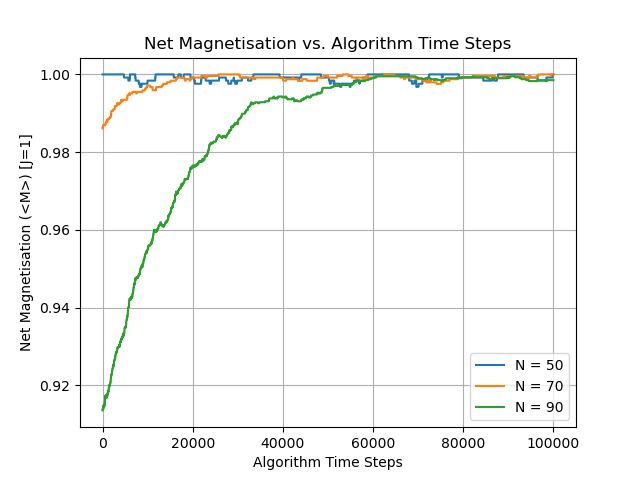
\includegraphics[width=\columnwidth]{metro_algobehaviour1.png}
    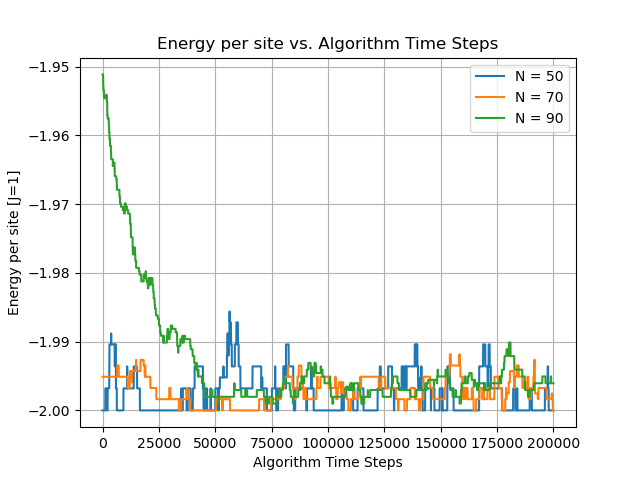
\includegraphics[width=\columnwidth]{metro_algobehaviour2.png}
    \caption{The first plot shows net magnetisation vs. algorithm time steps. The second plot shows energy per site vs. algorithm time steps. Both the plots are obtained with Metropolis algorithm. Here, $J = 1$ and $\beta = 1$.}
    \label{fig:metrobehaviour}
\end{figure}

\subsubsection{Net Magnetisation}
Fig.\ref{fig:metromag} shows the behaviour of net magnetisation with inverse temperature. The inverse temperature was varied between $0$ and $1$ with $70$ equally spaced points. The lattice sizes, $N = 50, 70, 90$ were studied. The plot also shows the expected analytical behaviour.
\begin{figure}[h!]
    \centering
    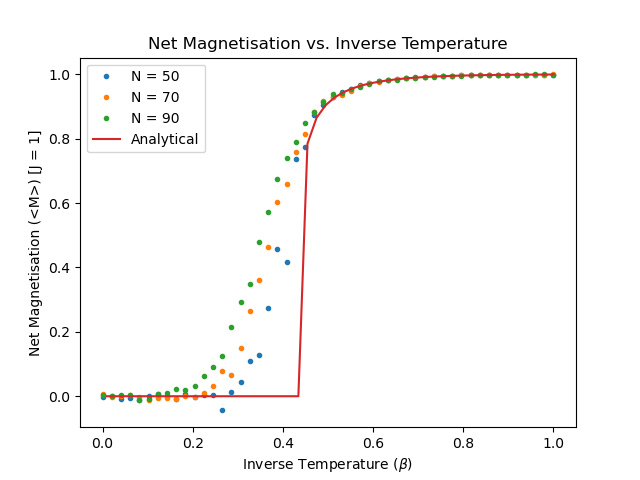
\includegraphics[width=\columnwidth]{metro_netmag-beta.png}
    \caption{Behaviour of net magnetisation with inverse temperature. Plot obtained with Metropolis algorithm and $J=1$.}
    \label{fig:metromag}
\end{figure}

\subsubsection{Susceptibility and Heat Capacity}
 Fig.\ref{fig:metrocchi} shows the behaviour of susceptibility and heat capacity. Again, the inverse temperature was varied between $0$ and $1$ with $70$ equally spaced points. The lattice sizes, $N = 50, 70, 90$ were studied. The plot shows the expected analytical behaviour of heat capacity. There is no closed form analytic solution for the behaviour of susceptibility \cite{suscep}.
\begin{figure}[h!]
    \centering
    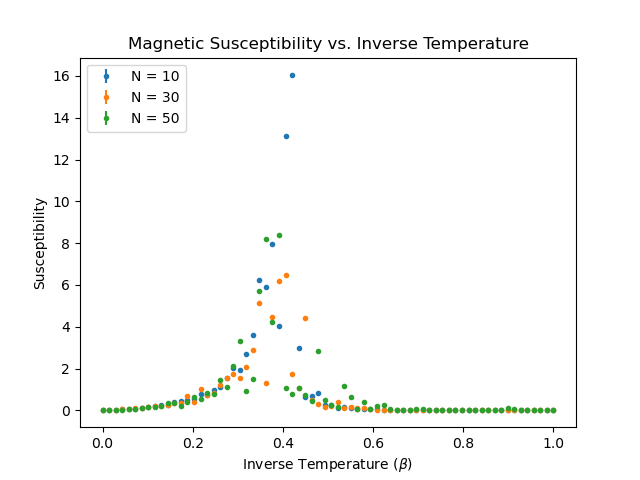
\includegraphics[width=\columnwidth]{metro_chi-beta.png}
    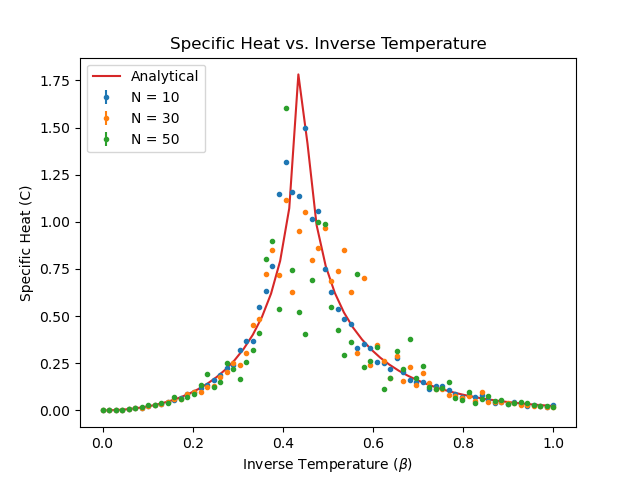
\includegraphics[width=\columnwidth]{metro_c-beta.png}
    \caption{Behaviour of magnetic susceptibility and heat capacity with inverse temperature. Plot obtained with Metropolis algorithm and $J=1$.}
    \label{fig:metrocchi}
\end{figure}

\subsubsection{Dynamical Critical Exponent}
Fig.\ref{fig:metrodyn} shows the behaviour of autocorrelation time with lattice size. The lattice size was varied between $5$ and $149$ at steps of $2$. The dynamical critical exponent is then extracted from the slope of the best linear fit to the $log-log$ plot.
\begin{figure}[h!]
    \centering
    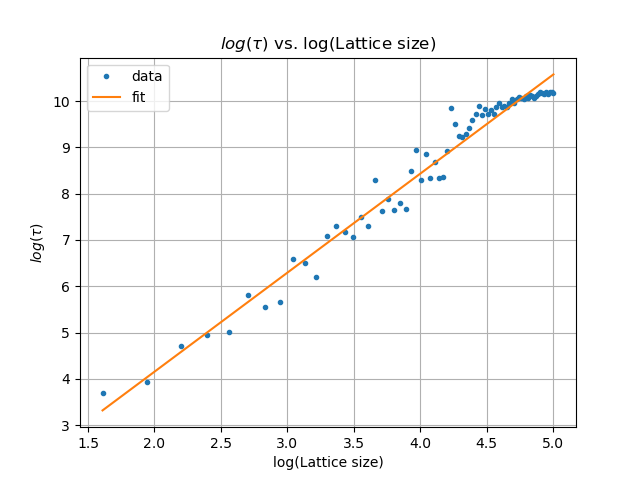
\includegraphics[width=\columnwidth]{metro_dyncritexp.png}
    \caption{Behaviour of autocorrelation time with lattice size. The best linear fit is also plotted, with a slope of $2.13$. This was obtained with Metropolis algorithm with $J=1$ and $\beta=1$.}
    \label{fig:metrodyn}
\end{figure}

\subsection{Worm Algorithm}
\subsubsection{Algorithm Behaviour}
Fig.\ref{fig:wormbehaviour} shows the behaviour of the Worm algorithm. Again, the initial configurations were lattices with sites set to $1$ with a probability of $0.8$ and sites set to $-1$ with a probability of $0.2$. This is neither a full cold-start nor a full hot-start, rather a mixture of the two. The plots do not include burn-in steps. The behaviour was studied with $100000$ iterations of the algorithm with $30000$ burn-in iterations, for a total of $130000$ iterations. The lattice sizes, $N = 50, 70, 90$ were studied.
\begin{figure}[h!]
    \centering
    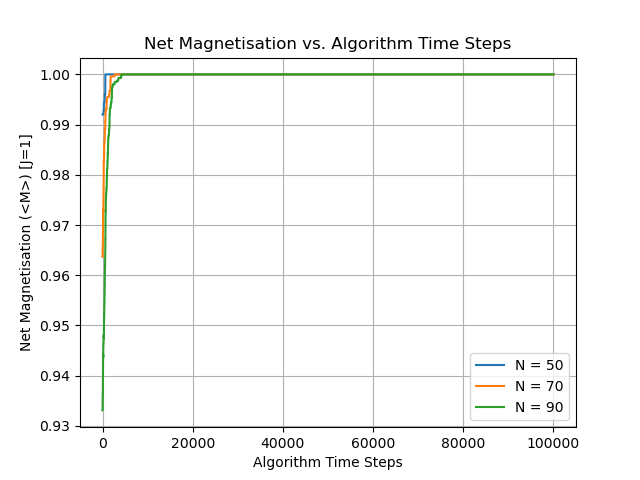
\includegraphics[width=\columnwidth]{worm_algobehaviour1.png}
    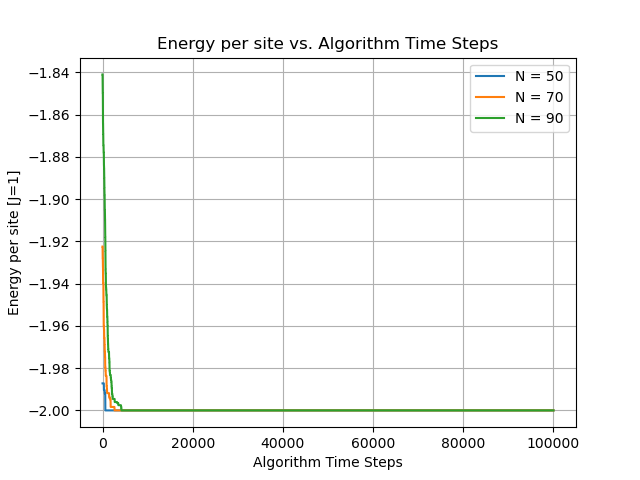
\includegraphics[width=\columnwidth]{worm_algobehaviour2.png}
    \caption{The first plot shows net magnetisation vs. algorithm time steps. The second plot shows energy per site vs. algorithm time steps. Both the plots are obtained with worm algorithm. Here, $J = 1$ and $\beta = 1$.}
    \label{fig:wormbehaviour}
\end{figure}

\subsubsection{Net Magnetisation}
Fig.\ref{fig:wormmag} shows the behaviour of net magnetisation with inverse temperature. The inverse temperature was varied between $0$ and $1$ with $70$ equally spaced points. The lattice sizes, $N = 50, 70, 90$ were studied. The plot also shows the expected analytical behaviour.
\begin{figure}[h!]
    \centering
    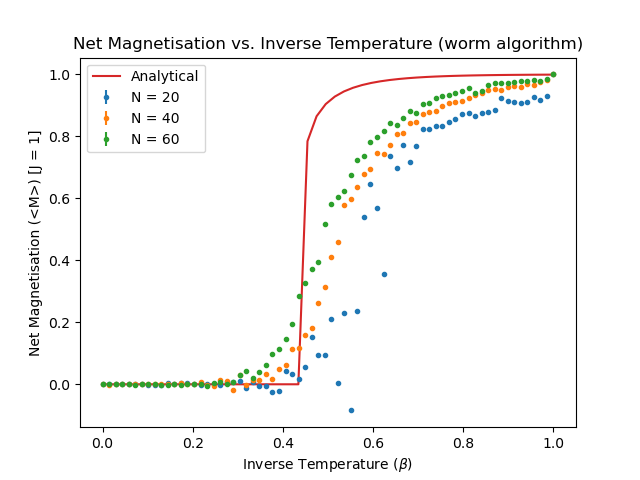
\includegraphics[width=\columnwidth]{worm_netmag-beta.png}
    \caption{Behaviour of net magnetisation with inverse temperature. Plot obtained with worm algorithm and $J=1$.}
    \label{fig:wormmag}
\end{figure}

\subsubsection{Susceptibility and Heat Capacity}
 Fig.\ref{fig:wormcchi} shows the behaviour of susceptibility and heat capacity. Again, the inverse temperature was varied between $0$ and $1$ with $70$ equally spaced points. The lattice sizes, $N = 10, 30, 50$ were studied. The plot shows the expected analytical behaviour of heat capacity. There is no closed form analytic solution for the behaviour of susceptibility \cite{suscep}.
\begin{figure}[h!]
    \centering
    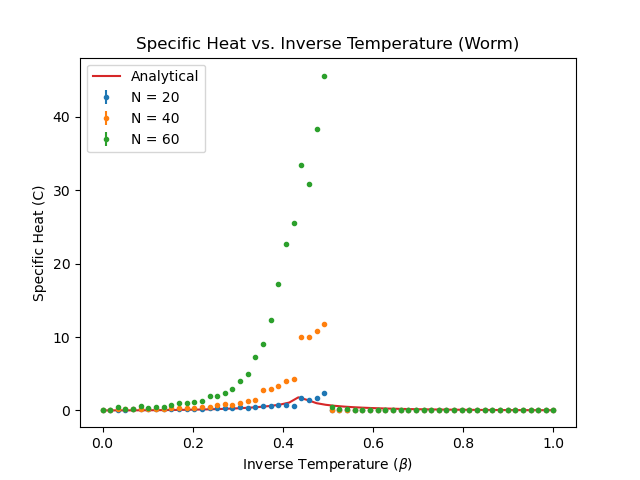
\includegraphics[width=\columnwidth]{worm_heat_1.png}
    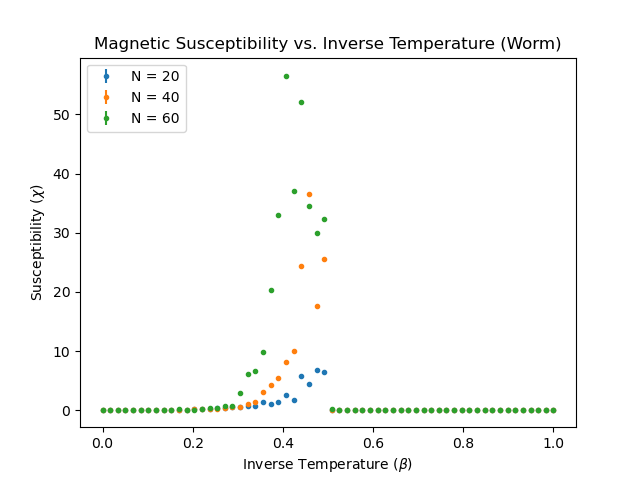
\includegraphics[width=\columnwidth]{worm_suscep.png}
    \caption{Behaviour of magnetic susceptibility and heat capacity with inverse temperature. Plot obtained with worm algorithm and $J=1$.}
    \label{fig:wormcchi}
\end{figure}

\subsubsection{Dynamical Critical Exponent}
Fig.\ref{fig:wormdyn} shows the behaviour of autocorrelation time with lattice size. The lattice size was varied between $5$ and $149$ at steps of $2$. The dynamical critical exponent is then extracted from the slope of the best linear fit to the $log-log$ plot.
\begin{figure}[h!]
    \centering
    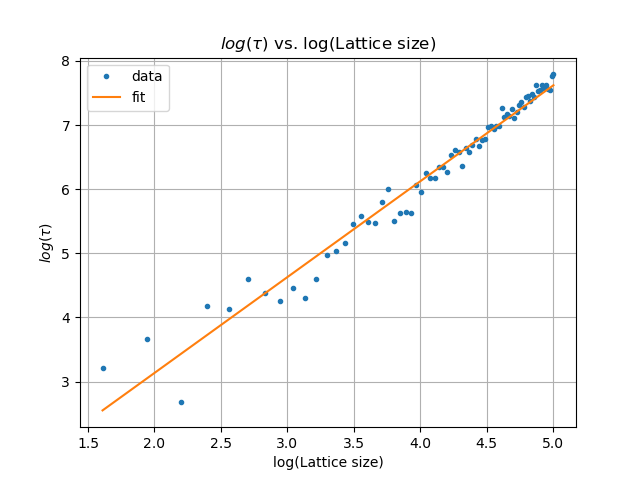
\includegraphics[width=\columnwidth]{worm_dyncritexp.png}
    \caption{Behaviour of autocorrelation time with lattice size. The best linear fit is also plotted, with a slope of $1.49$. This was obtained with Metropolis algorithm with $J=1$ and $\beta=1$.}
    \label{fig:wormdyn}
\end{figure}

\section{Discussion}
In the case of Metropolis algorithm, we see that the system takes longer to equilibrate with increase lattice sizes. This is not the case with worm algorithm, and this is what is expected, since worm algorithm is not a totally local algorithm. This is explicitly seen in the value of the critical dynamical exponent. In the case of Metropolis algorithm, fig.\ref{fig:metrodyn} shows a critical dynamical exponent of $2.13$. Over $20$ runs, the algorithm produced exponents in the range of $2.1$-$2.21$. This is comparable to the exponents in literature, $z \approx 2.2$\cite{metroexp}. Whereas, in the case of worm algorithm, fig.\ref{fig:wormdyn} shows a critical dynamical exponent of $1.49$. Over $20$ runs, the algorithm produced exponents in the range of $1.46$-$1.55$. This is lower than the value obtained with Metropolis algorithm. However, this is much higher than the value discussed in \cite{Prokof_ev_2001}. This can be attributed to the fact that we have not implemented exactly the variation of worm algorithm discussed in the paper. We would like to implement this particular method in the future and try to obtain the extremely low dynamical critical exponent discussed in the paper. One of the major drawbacks of our implementation, and something that we realised only much later, is that our implementation is not very efficient at low inverse temperatures or low interaction parameter values. This is intuitive now, since our algorithm grows the worm forever in such situations and gives the wrong result. However, this was overlooked, since we ran all our initial tests with the interaction parameter and inverse temperature set to $1$. To overcome this problem, we considered worms of alternating spins instead of same spins. This helped immensely in the low inverse temperature/low interaction parameter region. However, the behaviour of the observables were not exact. In fig.\ref{fig:wormmag} we see that the behaviour of the net magnetisation with inverse temperature improves with lattice size. Here, we had considered the other variation of the worm algorithm, where the worm consisted of alternating spins. The primary variation of the worm algorithm gave better results at high inverse temperatures, but suffered very much at low inverse temperatures. The behaviour of other observables, magnetic susceptibility and heat capacity, can be seen in fig.\ref{wormcchi}, and they show the expected behaviour of peaking at critical temperature. Although, we should notice that the behaviour given in the plots is not exact. It should be noted that the Metropolis algorithm gave slightly better results, see fig.\ref{fig:metrocchi}, however it was less efficient at large lattices. We state again that our implementation of worm algorithm is very suitable and powerful for large inverse temperatures. Therefore, the thing that we would like to do in the immediate future is to modify our implementation to behave reasonably at low inverse temperatures. We plan to do this by implementing the variation discussed by \cite{Prokof_ev_2001}. Unfortunately, 3D Ising model was not studied in this project. That would also be a good extension to the current project in the future.

\section{Summary}
To summarise, we implemented first studied the standard Metropolis algorithm and simulated 2D Ising model. Various observable and the dynamical critical exponent were calculated. We then implemented a variation of the worm algorithm, an alternative to the Metropolis algorithm. Again, various observable and the dynamical critical exponent were calculated. It was seen that the critical exponent in the case of the worm algorithm was much lower than the one calculated for the Metropolis algorithm. Further studies are required to implement other variations of the worm algorithm to further reduce the critical exponent and make this particular implementation better at low inverse temperatures.

\bibliography{reference}

\appendix
\begin{figure*}
    \centering
    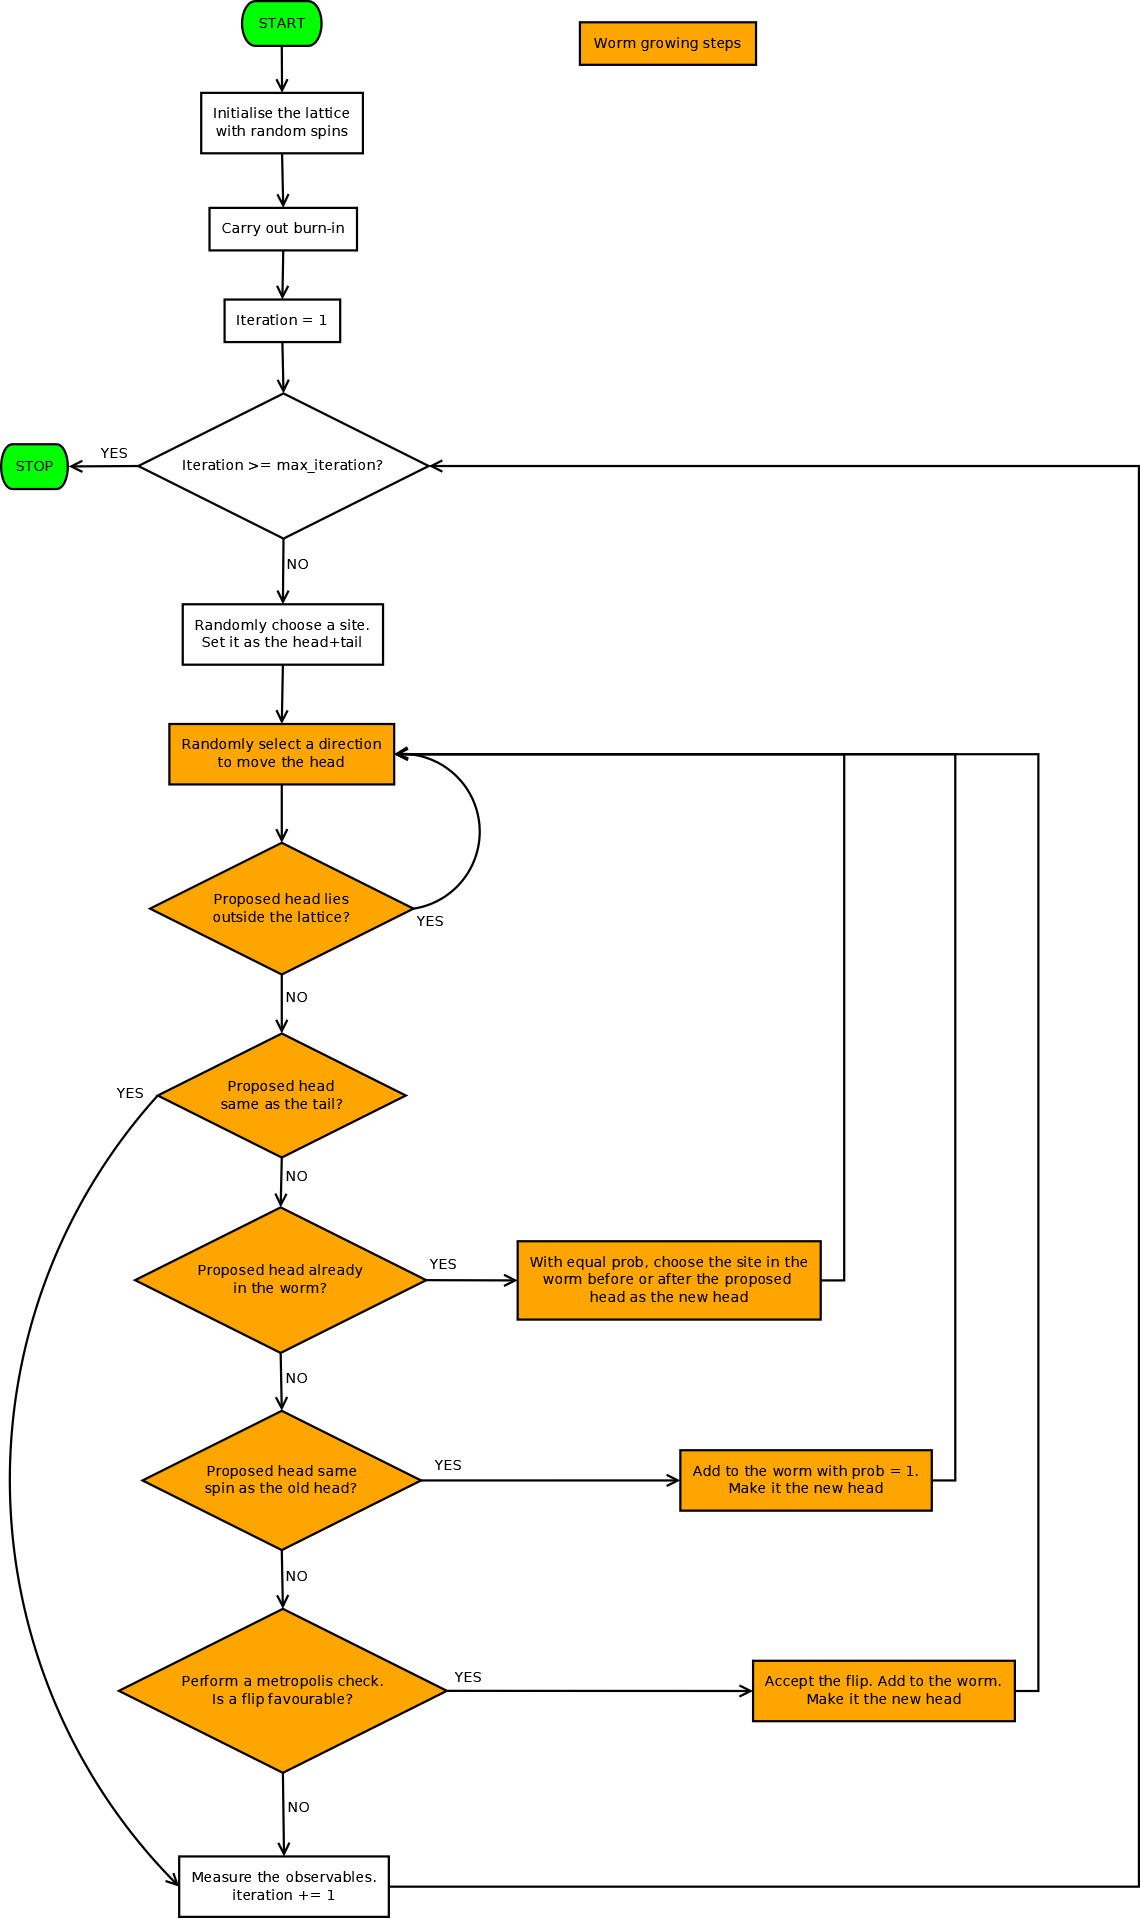
\includegraphics[scale=0.22]{worm_flowchart.png}
    \caption{The worm algorithm as implemented in this project.}
    \label{fig:flow}
\end{figure*}

\end{document}
